% remember to set these at the start of each chapter
\chapter{Background} 
\label{background} 

\section{Neural Networks}

The term Neural Network (NN) refers to a computational model that is artificially built in computers. The artificial Neural Network is inspired by the way biological neural networks in the human brain process information. Artificial Neural Networks have generated a lot of excitement in Machine Learning research and industry, thanks to many breakthrough results in speech recognition, computer vision and text processing. In this section, we will discuss the fundamentals of a Neural Network.

\subsection{A Single Neuron}
Neuron, or node, is a basic computation unit in NN. It simply takes some inputs $(x_1,...,x_n)$ and computes an output Y. Each input has an associated weight $(w_1,...,w_n)$, which is assigned on the basis of its relative importance to other inputs. The node applies a function $f$ to the weighted sum of its inputs (and a bias term $b$). The output of a node is $f(w_1 \cdot x_1 +...+ w_n \cdot x_n + b)$, shown in Fig.\,\ref{node}.
\begin{figure}
	\centering
	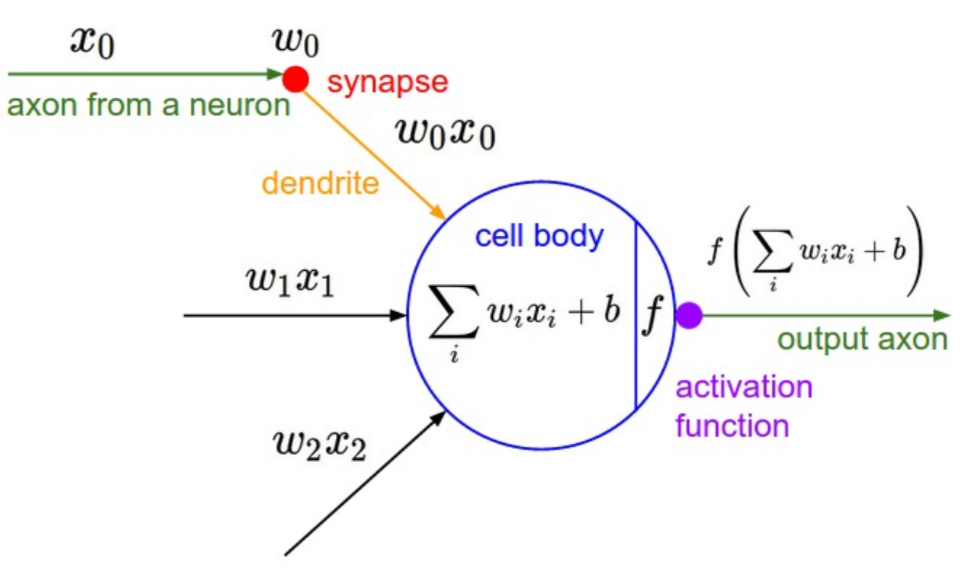
\includegraphics[scale=0.5]{Figs/node.png}
    \caption{A Node}
    \label{node}
\end{figure}

The function $f$ is non-linear and is called the Activation Function. The purpose of the activation function is to introduce non-linearity into the output of a node. The following activation function (Fig.\,\ref{activation}) is often used:
\begin{figure}
	\centering
	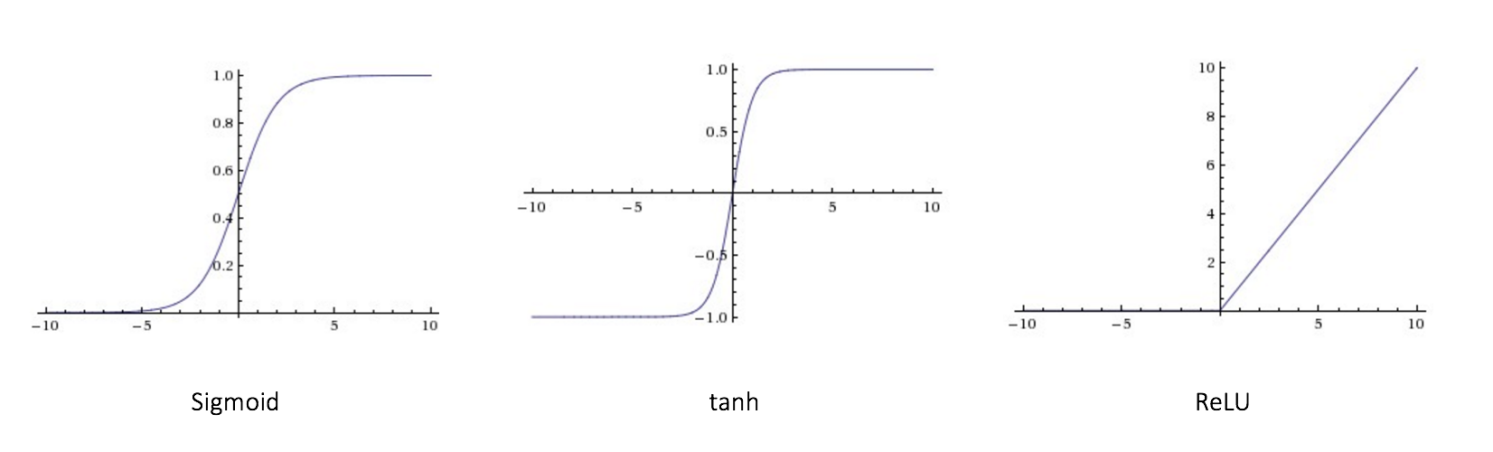
\includegraphics[scale=0.5]{Figs/activation.png}
    \caption{Activation Functions}
    \label{activation}
\end{figure}

\begin{itemize}
  \item Sigmoid: takes a real-valued input and squashes it to range between 0 and 1
        $$ \sigma(x) =  \frac{\mathrm{1} }{\mathrm{1} + e^{-x} }  $$ 
  \item tanh: takes a real-valued input and squashes it to the range [-1, 1]
        $$ tanh(x) = 2\cdot\sigma(2x)-1 $$
        
  \item ReLU(Rectified Linear Unit): takes a real-valued input and thresholds it at zero
        $$f(x) = \max(0,x)$$
\end{itemize}

\subsection{Feedforward Neural Network}
The feedforward neural network was the first and simplest type of artificial neural network devised [3]. It contains multiple neurons (nodes) arranged in layers. Nodes from adjacent layers have connections or edges between them. All these connections have weights associated with them.

An example of a feedforward neural network is shown in Fig.\,\ref{feedforward}.
\begin{figure}
	\centering
	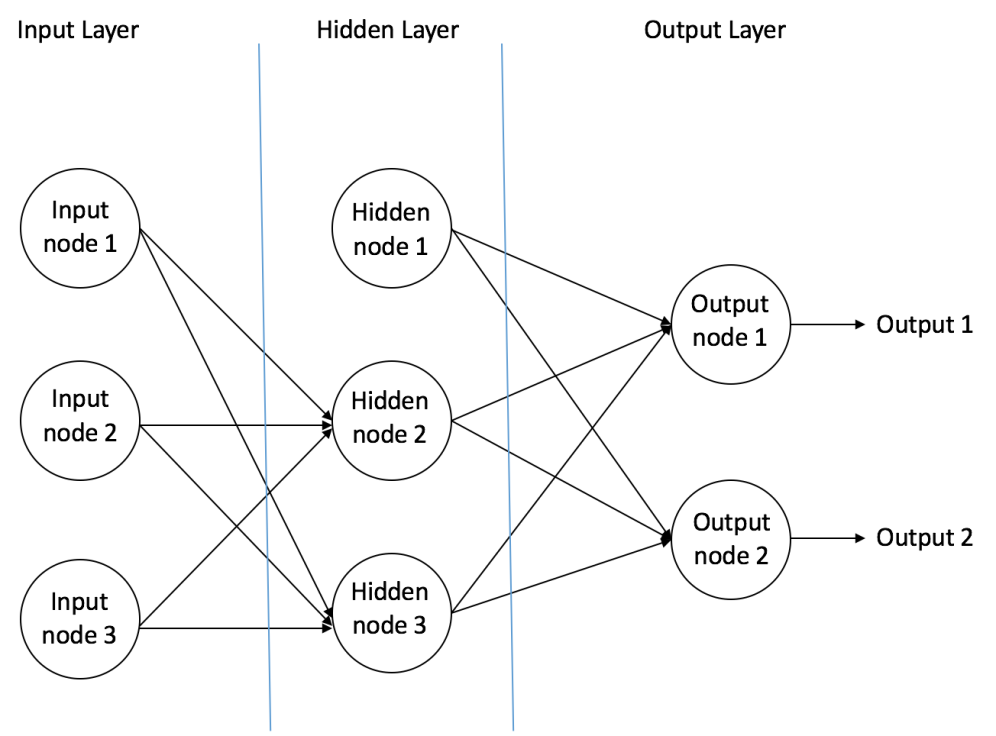
\includegraphics[scale=0.5]{Figs/feedforward.png}
    \caption{Feedforward Neural Network}
    \label{feedforward}
\end{figure}

A feedforward neural network can consist of three types of nodes:

\begin{enumerate}
\item Input Nodes – The Input nodes provide information from the outside world to the network and are   together referred to as the “Input Layer”. No computation is performed in any of the Input nodes – they just pass on the information to the hidden nodes.
\item Hidden Nodes – The Hidden nodes have no direct connection with the outside world (hence the name “hidden”). They perform computations and transfer information from the input nodes to the output nodes. A collection of hidden nodes forms a “Hidden Layer”. While a feedforward network will only have a single input layer and a single output layer, it can have zero or multiple Hidden Layers.
\item Output Nodes – The Output nodes are collectively referred to as the “Output Layer” and are responsible for computations and transferring information from the network to the outside world.
\end{enumerate}

In a feedforward network, the information moves in only one direction – forward – from the input nodes, through the hidden nodes (if any) and to the output nodes. There are no cycles or loops in the network


\subsection{Multi Layer Perceptron}
\subsection{Back-Propagation}




\section{Convolutional Neural Networks}
\subsection{Convolution Layer — The Kernel}
\subsection{Pooling Layer}
\subsection{Classification — Fully Connected Layer (FC Layer)}
\section{K-Fold Cross Validation}
\section{Image data augmentation}



